\documentclass{ctexart}
\usepackage{amsmath}
\usepackage{geometry}
\usepackage{hyperref}
\usepackage{graphicx}
\usepackage{subfigure}
\usepackage{float}
\title{用示波器观测动态磁滞回线}
\author{陈启钰\,\,\,2300011447}
\date{\today}
\begin{document}
	\maketitle
	\tableofcontents
	\section{观测铁氧体的磁滞回线}
	\subsection{$100\mathrm{Hz}$下铁氧体饱和磁滞回线的测量结果}
	本部分中的各参量值为$R_1=2.0\mathrm{\Omega},R_2=50\mathrm{k\Omega},C=10.0\mathrm{\mu F},f=100\mathrm{Hz}$,用示波器两通道测量$R_1$以及$C$两端电压,得到的数据如下表
	\begin{table}[H]
		\begin{center}
			\caption{$100\mathrm{Hz}$下铁氧体饱和磁滞回线测量记录表}
			\begin{tabular}{c|cccccccccc}
				$u_{R_1}/\mathrm{mV}$&-36.0&0.00&48.0&100&299&356&201&100&65.0&50.0\\
				\hline
				$u_{C}/\mathrm{mV}$ &0.00 &5.50 &10.2 &12.3 &14.3 &14.4 &13.3 &9.20 &4.10 & 1.90\\
				\hline
				$u_{R_1}/\mathrm{mV}$ &37.0&0.00 &-56.0 &-100 &-300 &-333 &-262 &-109 &-72.0 &-50.0 \\
				\hline
				$u_{C}/\mathrm{mV}$ &0.00 &-5.60 &-10.0 &-11.7 &-13.5 &-14.1 &-14.0 &-9.90 &-6.10 &-2.30 \\
			\end{tabular}
		\end{center}
	\end{table}
	通过公式
	\begin{align}
		B=\frac{R_2C}{N_2S}u_C\\
		H=\frac{N_1}{lR_1}u_{R_1}
	\end{align}
	可以计算出所对应的磁感应强度和磁场强度,作图如下
	\begin{figure}[H]
		\centering
		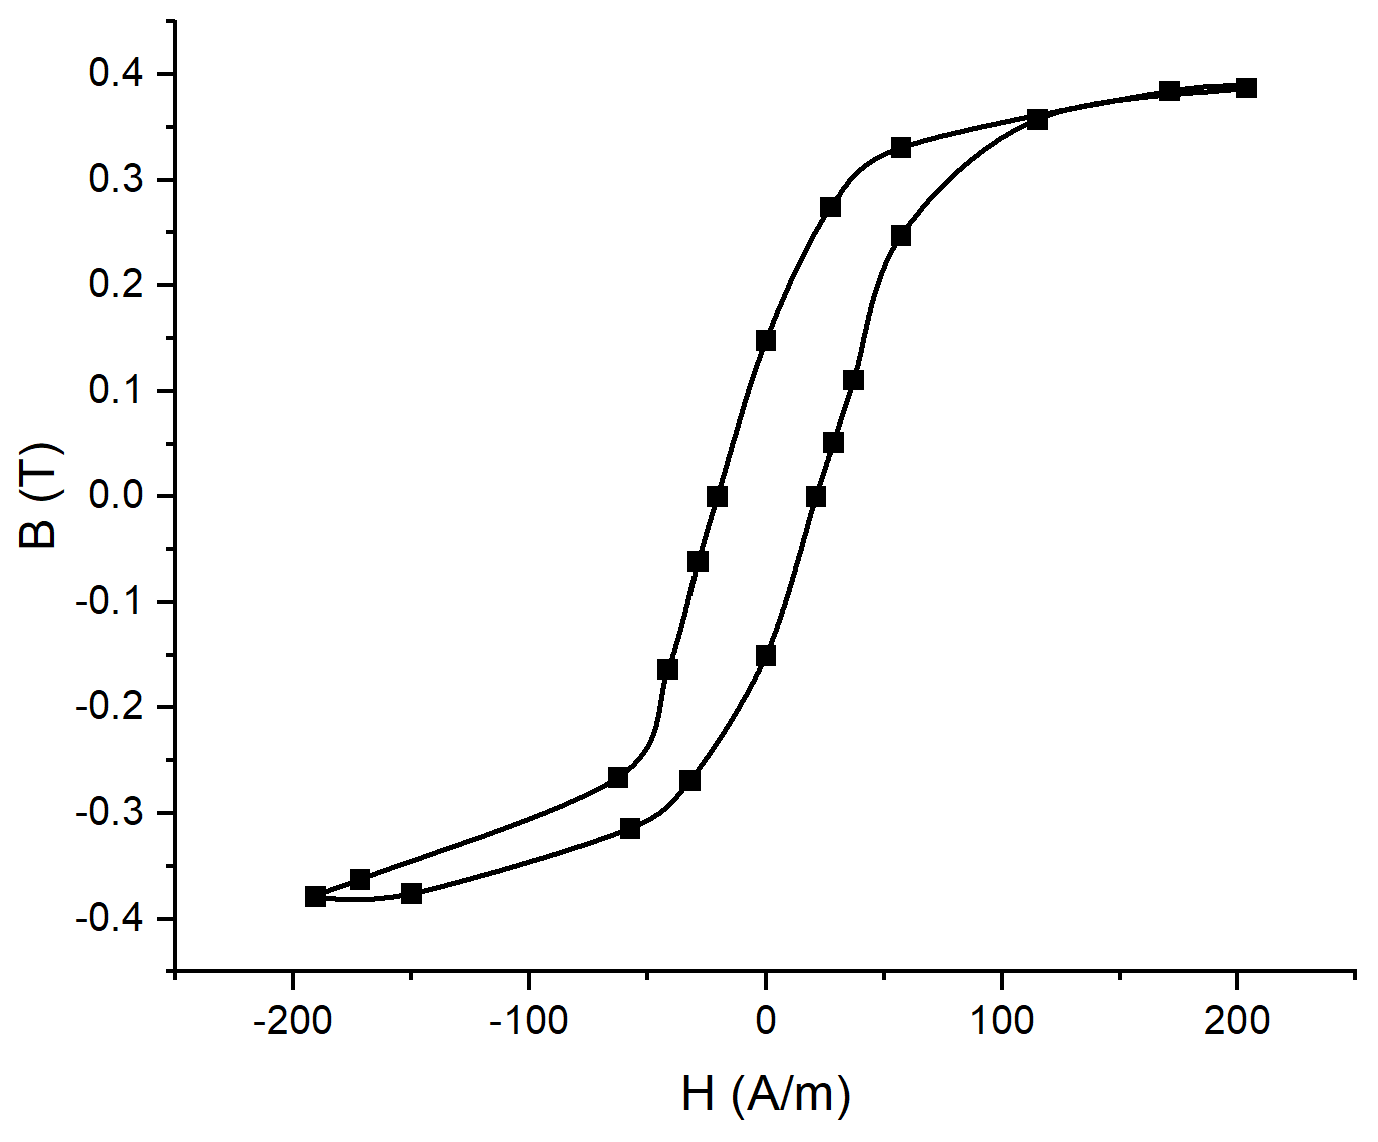
\includegraphics[width=8cm]{1.png}
		\caption{铁氧体的饱和磁滞回线图}
	\end{figure}
	可以计算得到
	\begin{align}
		B_S=0.387\mathrm{T}\\
		B_r=0.148\mathrm{T}\\
		H_c=20.8\mathrm{A/m}
	\end{align}
	\subsection{$50\mathrm{Hz}$、$150\mathrm{Hz}$时$B_r$以及$H_c$的测量}
	当$f=50\mathrm{Hz}$时,测得
	\begin{align}
		u_{C_r}=8.20\mathrm{mV},u_{R_1c}=55.0\mathrm{mV}
	\end{align}
	不确定度
	\begin{align}
		\sigma_{u_{C_r}}=8.20\mathrm{mV}\times 2\%+50\mathrm{mV}\times 0.3\%=0.32\mathrm{mV}\\
		\sigma_{u_{R_1c}}=55.0\mathrm{mV}\times 2\%+500\mathrm{mV}\times0.3\%=2.6\mathrm{mV}
	\end{align}
	可以算出
	\begin{align}
		B_r=(0.220\pm0.009)\mathrm{T},H_c=(31.7\pm 1.5)\mathrm{A/m}
	\end{align}
	同样的,当$f=150\mathrm{Hz}$时
	\begin{align}
		u_{C_r}=3.50\mathrm{mV},u_{R_1c}=25.0\mathrm{mV}
	\end{align}
	不确定度计算同理,在此略去,最后算出
	\begin{align}
		B_r=(0.094\pm0.004)\mathrm{T},H_c=(14.4\pm1.0)\mathrm{A/m}
	\end{align}
	可见,随着频率的增加,$B_r$和$H_c$都会变小。对为什么会变小的讨论放在和硅钢合金一起,见第四部分。
	\subsection{不同时间常数下的李萨如图形}
	通过改变时间常数$\tau=R_2C$,我们得到不同情况下的李萨如图形,如下图所示
	\begin{figure}[H]
		\centering
		\subfigure[$\tau=0.01\mathrm{s}$]{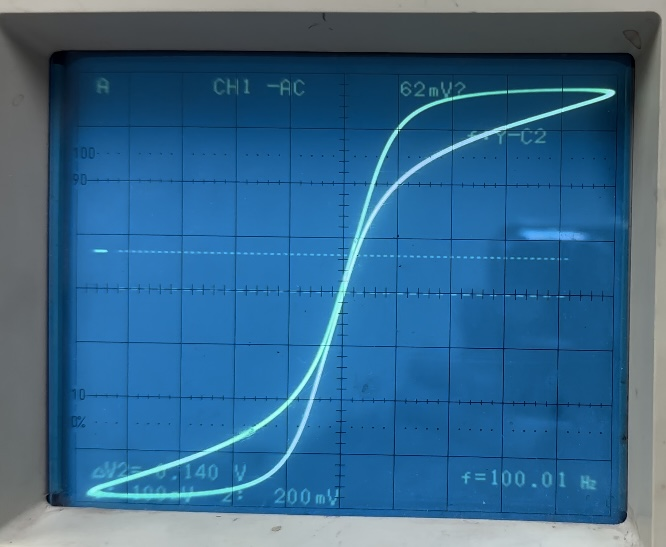
\includegraphics[width=5cm]{p1.jpg}}
		\subfigure[$\tau=0.05\mathrm{s}$]{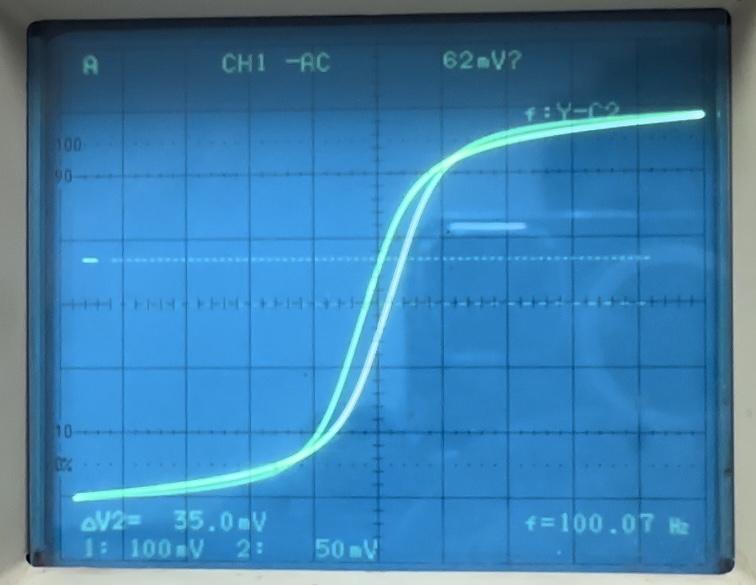
\includegraphics[width=5cm]{p2.jpg}}
	\end{figure}
	\begin{figure}[H]
		\centering
		\subfigure[$\tau=0.5\mathrm{s}$]{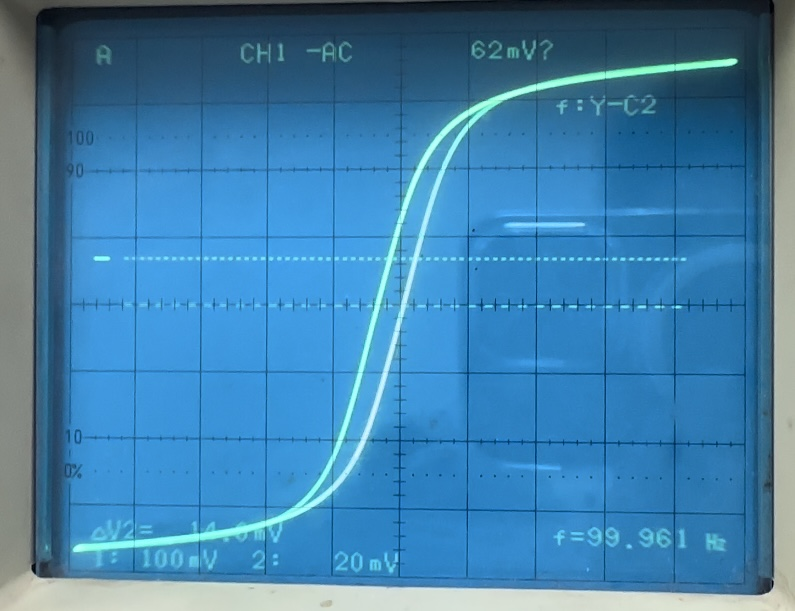
\includegraphics[width=5cm]{p3.jpg}}
		\caption{不同时间常数下的磁滞回线}
	\end{figure}
	这是是因为随着时间常数改变,导致积分电路满足的条件不满足,从而我们看到的李萨如图形也会改变。
	\section{测量铁氧体的动态磁化曲线}
	本部分中的参量设置为$f=100\mathrm{Hz},R_1=2.0\mathrm{\Omega},R_2=50\mathrm{k\Omega},C=10\mathrm{\mu F}$,通过改变励磁电流,可以测得示波器上李萨如图形顶点对应的两个电压值
	\begin{table}[H]
		\begin{center}
			\caption{$100\mathrm{Hz}$下铁氧体动态磁化曲线测量记录表}
			\begin{tabular}{c|cccccccccc}
				$u_{R_1}/\mathrm{mV}$ &16.1 &21.0 &35.0 &47.0 &60.0 &67.0 &83.0 &95.0 &109 &128 \\
				\hline
				$u_{C}/\mathrm{mV}$ &1.60 &2.10 &3.50 &4.70 &6.30 &7.10 &8.60 &9.50 &10.6 &11.3 \\
				\hline
				$u_{R_1}/\mathrm{mV}$ &135 &150 &174 &197 &228 &252 &274 &303 &340 &371 \\
				\hline
				$u_{C}/\mathrm{mV}$ &11.5 &12.0 &12.6 &13.0 &13.2 &13.5 &13.6 &13.8 &14.0 &14.1 \\
				\hline
				$u_{R_1}/\mathrm{mV}$&421&440&472&521&572&600&&&&\\
				\hline
				$u_{C}/\mathrm{mV}$&14.2&14.3&14.4&14.4&14.4&14.4&&&&
			\end{tabular}
		\end{center}
	\end{table}
	仍然根据公式
	\begin{align}
		H_m=\frac{N_1}{lR_1}u_{R_1}\\
		B_m=\frac{R_2C}{N_2S}u_C
	\end{align}
	以及
	\begin{align}
		\mu_m=\frac{B_m}{\mu_0H_m}
	\end{align}
	列表如下
		\begin{table}[H]
		\begin{center}
			\caption{$\mu_m-H_m$关系}
			\begin{tabular}{c|cccccccccc}
				$H_m/\mathrm{A/m}$&9.23&12.1
				&20.2				&27.1
				&34.6			&38.7
				&47.9				&54.8
				&62.9				&73.8
				\\ \hline
				$\mu_m$&3685&
				3708&
				3708&
				3708&
				3893&
				3929&
				3841&
				3707&
				3606&
				3273
				\\ \hline
				$H_m/\mathrm{A/m}$&
				77.9&
				86.5&
				100.4&
				113.7&
				131.5&
				145.4&
				158.1&
				174.8&
				196.2&
				214.0\\ \hline
				$\mu_m$&
				3159&
				2966&
				2685&
				2446&
				2147&
				1986&
				1840&
				1689&
				1527&
				1409\\ \hline
				$H_m/\mathrm{A/m}$&
				242.9&
				253.4&
				272.3&
				300.6&
				330.0&
				346.2&&&&\\ \hline
				$\mu_m$&
				1251&
				1205&
				1131&
				1024&
				933.5&
				889.9&&&&
			\end{tabular}
		\end{center}
	\end{table}
	可画出$\mu_m-H_m$曲线
	\begin{figure}[H]
		\centering
		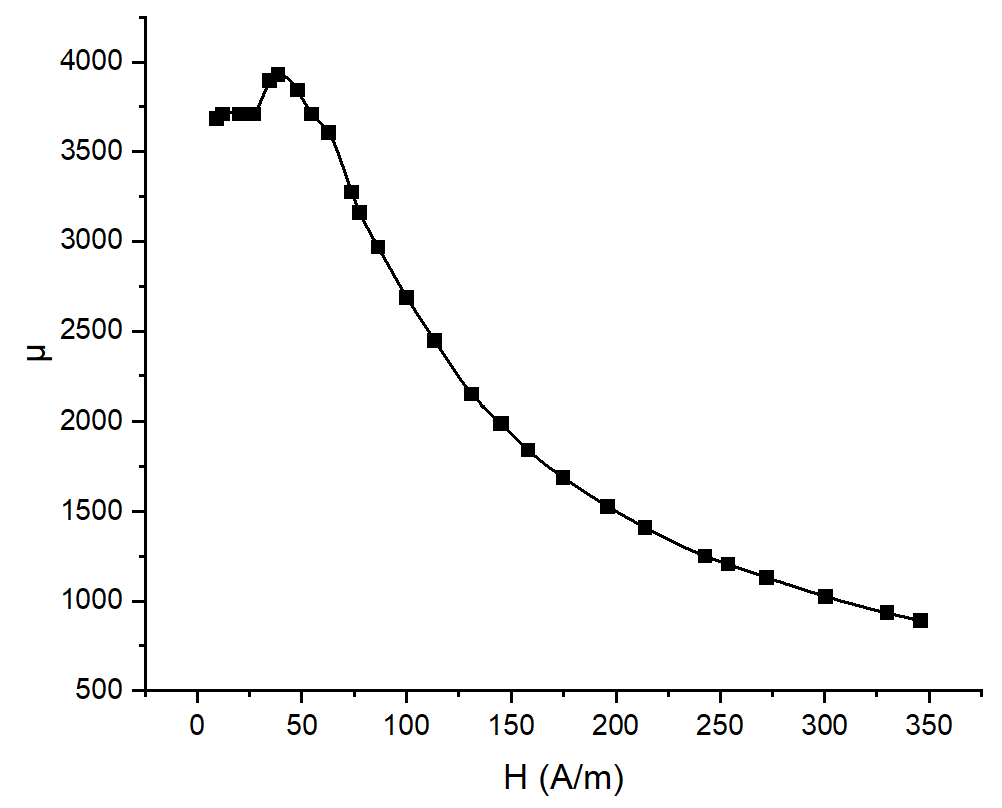
\includegraphics[width=8cm]{2.png}
		\caption{$\mu_m-H_m$曲线图}
	\end{figure}
	\section{测量铁氧体的可逆磁导率以及起始磁导率}
	本部分参量设置为$R_1=2\mathrm{\Omega},R_2=20\mathrm{k\Omega},C=2.0\mathrm{\mu F},f=100\mathrm{Hz}$
	实验数据列表如下
	\begin{table}[H]
		\begin{center}
			\caption{有直流偏置时的可逆磁导率测量结果}
			\begin{tabular}{c|cccccccccc}
				$I/\mathrm{A}$&0.000&0.021&0.040&0.060&0.080&0.100&0.120&0.140&0.160&0.180\\\hline
				$\Delta u_C/\mathrm{mV}$&3.95&3.95&3.80&3.00&2.10&1.50&1.15&0.900&0.750&0.600\\\hline
				$\Delta u_{R_1}/\mathrm{mV}$&5.40&6.60&10.05&12.65&13.80&13.80&13.50&13.20&13.10&12.90
			\end{tabular}
		\end{center}
	\end{table}
	直流偏置磁场
	\begin{align}
		H=\frac{N_3}{l}I
	\end{align}
	而可逆磁导率
	\begin{align}
		\mu_R=\lim_{\Delta H\rightarrow0}\frac{\Delta B}{\mu_0 \Delta H}
	\end{align}
	最后可画出$\mu_R-H$图像如下
	\begin{figure}[H]
		\centering
		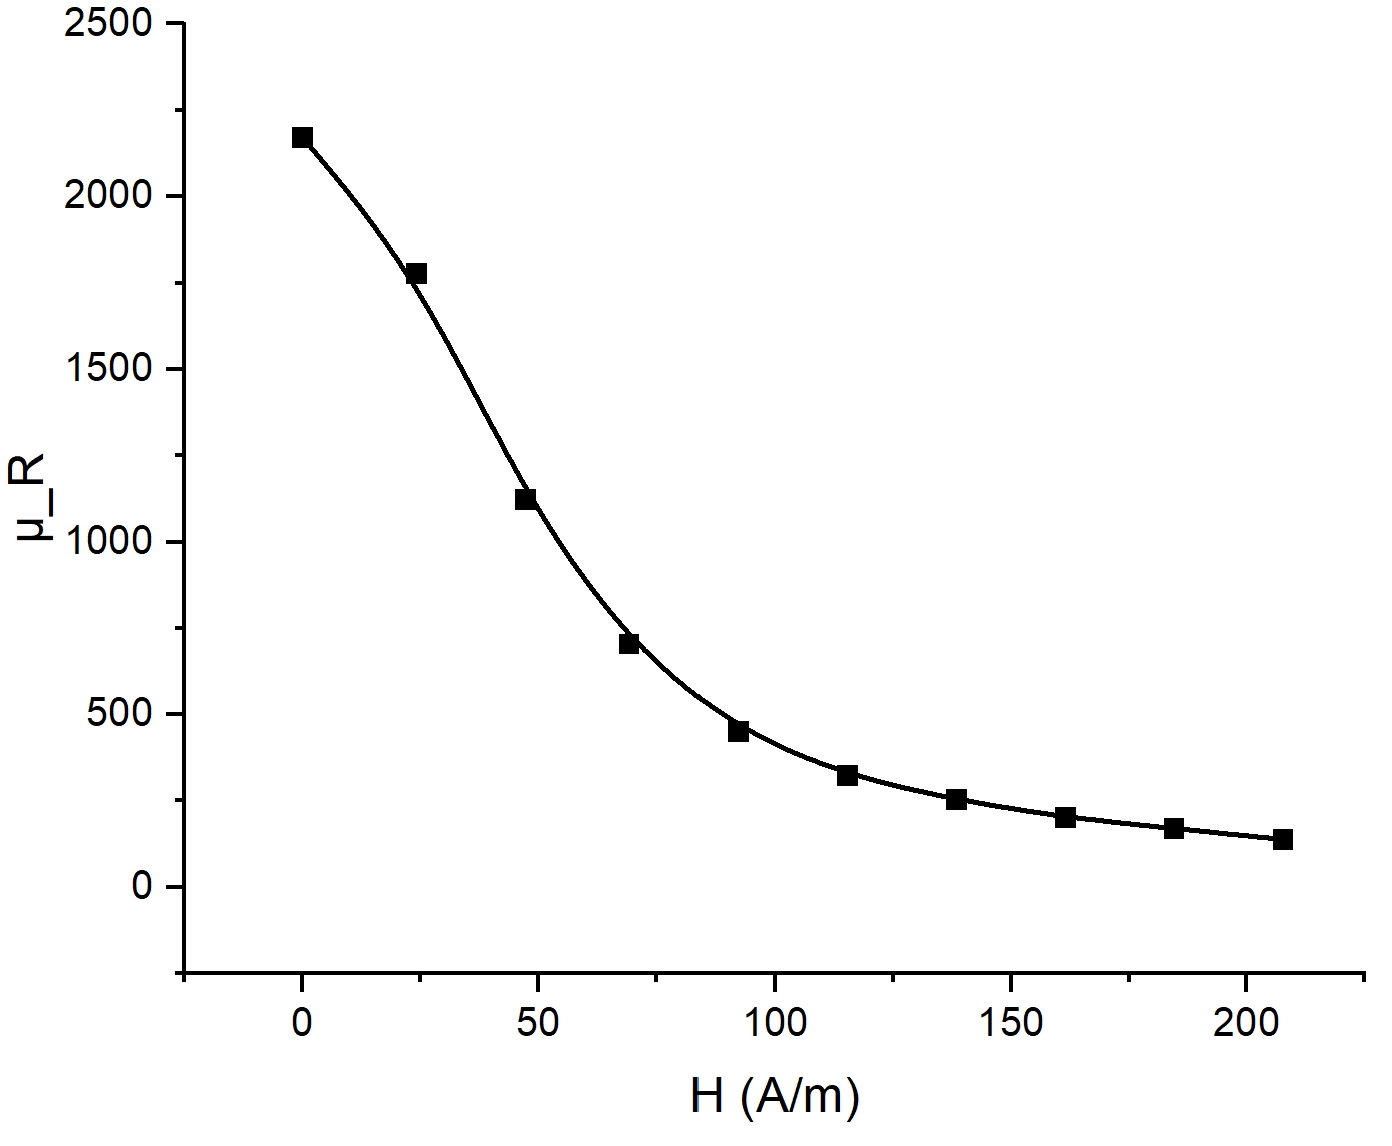
\includegraphics[width=8cm]{3.png}
		\caption{$\mu_R-H$图像}
	\end{figure}
	起始磁导率即$H=0$时的磁导率,根据数据可知
	\begin{align}
		\mu_i=2.17\times10^3
	\end{align}
	\section{给定交变磁场幅度下硅钢的磁滞回线变化规律}
	本部分参数$R_1=2.0\mathrm{\Omega},R_2=50\mathrm{k\Omega},C=10\mu F$。当$H_m$给定为$400\mathrm{A/m}$时,可算出$u_{R_1}=0.400\mathrm{V}$,实验数据记录如下
	\begin{table}[H]
		\begin{center}
			\caption{硅钢的磁滞回线变化规律数据记录表}
			\begin{tabular}{c|ccc}
				$f/\mathrm{Hz}$&20&40&60\\\hline
				$u_{Cm}/\mathrm{mV}$&33.2&33.0&33.0\\\hline
				$u_{Cr}/\mathrm{mV}$&20.8&22.0&22.8\\\hline
				$u_{R_1c}/\mathrm{mV}$&99.0&117&137
			\end{tabular}
		\end{center}
	\end{table}
	所对应的$B_m,B_r,H_c$则在下表中呈现
	\begin{table}[H]
		\begin{center}
			\caption{给定交变磁场幅度下硅钢的磁滞回线变化规律}
			\begin{tabular}{c|ccc}
				$f/\mathrm{Hz}$&20&40&60\\\hline
				$B_m/\mathrm{T}$&0.922&0.917&0.917\\\hline
				$B_r/\mathrm{T}$&0.578&0.611&0.633\\\hline
				$H_c/\mathrm{A/m}$&99.0&117&137
			\end{tabular}
		\end{center}
	\end{table}
	可见,随频率增大,$B_m$变化不明显,但$B_r,H_c$都会增加。
	我们可以看到,随着频率的增加,对于铁氧体来说,$B_r$和$H_c$会增大,而对于硅钢合金来说,$B_r$和$H_c$会变小。矫顽力随频率变化的原因可能是磁畴在反向磁场下因热产生的效应以及磁粘滞系数\footnote{参考维基百科}。所以会出现不同材料矫顽力随频率变化的不同的情况,这取决于材料的特性。还有一个猜测是铁氧体和硅钢随着频率增加一个涡流增加,一个涡流减小(对应)。
	\section{原始数据}
	实验的原始数据通过图片的形式附在最后
	\begin{figure}[H]
		\centering
		\includegraphics[width=16cm,angle=270]{da1.jpg}
	\end{figure}
	\begin{figure}[H]
		\centering
		\includegraphics[width=16cm,angle=270]{da2.jpg}
	\end{figure}
	\begin{figure}[H]
		\centering
		\includegraphics[width=16cm,angle=270]{da3.jpg}
	\end{figure}
\end{document}